\documentclass[spanish,xcolor={table}]{beamer}

\usepackage[utf8]{inputenc}

\usepackage[spanish,activeacute]{babel}
\spanishplainpercent
\uselanguage{Spanish}
\languagepath{Spanish}

\usepackage{lmodern}
\usepackage{libertineRoman}
\usepackage{biolinum}
\usepackage{eulervm}
\usepackage[T1]{fontenc}
\usepackage[normalem]{ulem}

\usepackage{amsmath,amssymb,amsthm,mathtools,mathabx}
\usepackage[italic,nolessnomore]{mathastext}

\usepackage{tikz}
\usetikzlibrary{arrows}
\usetikzlibrary{babel}
\usetikzlibrary{overlay-beamer-styles}
\usepackage{pgfplots}
\pgfplotsset{compat=1.9}
\pgfkeys{/pgf/number format/1000 sep={$.$}}
\pgfkeys{/pgf/number format/dec sep={$,$}}

\usepackage{multicol}
\usepackage{tabularx}
\newcolumntype{C}{>{\centering\arraybackslash}X}
\usepackage{diagbox}

\newcommand\wider[2][3em]{%
\makebox[\linewidth][c]{%
  \begin{minipage}{\dimexpr\textwidth+#1\relax}
  \raggedright#2
  \end{minipage}%
  }%
}

% ----------------------------------------------------------------------------

% Beamer settings
\useoutertheme{default}
\useinnertheme{rectangles}
\usefonttheme[onlymath]{serif}
\setbeamertemplate{blocks}[rounded]
\beamertemplatenavigationsymbolsempty

% Paragraph spacing
\setlength{\parskip}{.5em}

% Item spacing
\usepackage{etoolbox}
\makeatletter
\patchcmd{\@listI}{\itemsep3\p@}{\itemsep6\p@}{}{}
\patchcmd{\@listii}{\itemsep\parsep}{\itemsep3\p@}{}{}
\makeatother

% Remove figure caption prefix
\setbeamertemplate{caption}{\raggedright\insertcaption\par}

% ----------------------------------------------------------------------------

% \DeclareTextFontCommand{\emph}{\bfseries}

\theoremstyle{plain}
\newtheorem{theorem}{Teorema}
\newtheorem{proposition}[theorem]{Proposición}
\newtheorem{corollary}[theorem]{Corolario}
\newtheorem{lemma}[theorem]{Lema}
\newtheorem*{theorem*}{Teorema}
\newtheorem*{proposition*}{Proposición}
\newtheorem*{corollary*}{Corolario}
\newtheorem*{lemma*}{Lema}

\theoremstyle{definition}
\newtheorem{definition}{Definición}

\theoremstyle{remark}
\newtheorem*{remark}{Observación}
\newtheorem*{example}{Ejemplo}
\newtheorem*{examples}{Ejemplos}

\newcommand{\note}[1]{\textbf{\textcolor{red}{#1}}}
\newcommand{\pending}[1]{\textbf{\textcolor{blue}{#1}}}

\newcommand{\alphabet}{\ensuremath{\mathcal{A}}}
\newcommand{\nats}{\ensuremath{\mathbb{N}}}

\newcommand{\neck}[1]{\left[#1\right]}
\newcommand{\substr}[2]{_{[#1\,..\,#2]}}

\newcommand{\mat}[1]{\mathbf{#1}}

\newcommand{\Succ}[1]{\ensuremath{\text{S}_{#1}}}
\newcommand{\Pred}[1]{\ensuremath{\text{P}_{#1}}}

\newcommand{\laplacian}{\ensuremath{\operatorname{L}}}
\newcommand{\determinant}{\ensuremath{\operatorname{det}}}
\newcommand{\edges}{\ensuremath{\operatorname{E}}}

\newcommand{\DB}[1]{\ensuremath{\text{DB}_{#1}}}
\newcommand{\M}[2]{\ensuremath{\text{M}_{#1}^{#2}}}
\newcommand{\NM}[2]{\ensuremath{\text{NM}_{#1}^{#2}}}
\newcommand{\Pf}[2]{\ensuremath{\text{P}_{#1}^{#2}}}
\newcommand{\NPf}[2]{\ensuremath{\text{NP}_{#1}^{#2}}}

\newcommand{\BEST}{\mdseries\textsc{best}}

\DeclareTextFontCommand{\emph}{\bfseries}

\definecolor{ne-proof}{HTML}{ea5c69}
\definecolor{ne-empir}{HTML}{ffac81}
\definecolor{ne-conjc}{HTML}{fdf2ac}
\definecolor{e-count-for}{HTML}{58d383}
\definecolor{e-count-emp}{HTML}{71d7e9}
\definecolor{e-examples}{HTML}{d9edfa}

% ----------------------------------------------------------------------------

\title{Secuencias maravillosas anidadas}
\subtitle{Tesis de Licenciatura en Ciencias de la Computación}
\author{Franco Frizzo}
\institute[DC, FCEyN, UBA]
    {Departamento de Computación, FCEyN, UBA}
\date{28 de diciembre de 2020}

% ============================================================================

\begin{document}

\frame{\titlepage}

% ============================================================================

\begin{frame}{Preliminares}

\begin{itemize}
  \item Trabajaremos con un \emph{alfabeto} de $b$ símbolos ($b > 2$).
  \begin{itemize}
    \item En los ejemplos, $b = 2$, $\alphabet = \lbrace 0, 1 \rbrace$.
  \end{itemize}
  \pause
  
  \item Una \emph{palabra} (o cadena, o secuencia) es una tira de símbolos de este alfabeto.
  
  \begin{example}
    11100 es una palabra sobre $\alphabet = \lbrace 0, 1 \rbrace$.
  \end{example}
  \pause
  
  \item Un \emph{collar} es una palabra mirada circularmente. \\
  Podemos pensarlo como el conjunto de rotaciones de una palabra.
  
  \begin{example}
    $\neck{11100} = \lbrace 11100, 01110, 00111, 10011, 11001 \rbrace$.
  \end{example}
  \pause
  
  \item Un \emph{corte} de un collar es cada una de las palabras que forman
  parte del mismo.
\end{itemize}

\end{frame}

% ----------------------------------------------------------------------------

\begin{frame}<-11>{Collares y secuencias de De~Bruijn}
  
  \begin{columns}
    \column{.4\textwidth - 1cm}
    \begin{figure}
      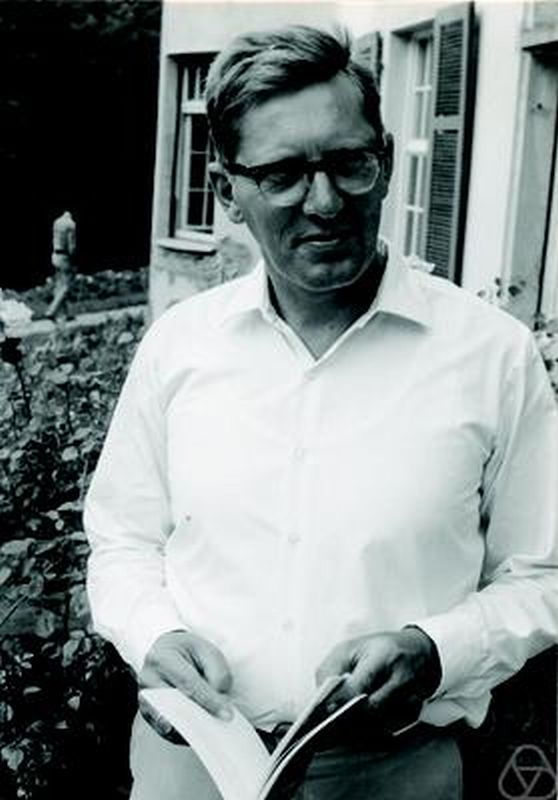
\includegraphics[width=\textwidth]{de-bruijn.jpg}
      \caption{Nicolaas G. de~Bruijn}
  \end{figure}
  \column{.6\textwidth}
  
  \begin{definition}
    Un \emph{collar de De~Bruijn} de orden $n$ es un collar de longitud
    $b^n$ donde cada palabra de longitud $n$ aparece una vez.
    
    \medskip
    
    Una \emph{secuencia de De~Bruijn} es un corte de un collar de De~Bruijn.
  \end{definition}
  \pause
  
  \begin{example}
    Tomemos $n = 3$. \vspace{-.5em}
    
    \begin{multicols}{2}
      \begin{tabular}{ll}
        \alt<5->{\alt<5>{\textcolor{red}{000}}{\sout{000}}}{000} &
        \alt<4->{\alt<4>{\textcolor{red}{100}}{\sout{100}}}{100} \\
        \alt<6->{\alt<6>{\textcolor{red}{001}}{\sout{001}}}{001} &
        \alt<8->{\alt<8>{\textcolor{red}{101}}{\sout{101}}}{101} \\
        \alt<7->{\alt<7>{\textcolor{red}{010}}{\sout{010}}}{010} &
        \alt<3->{\alt<3>{\textcolor{red}{110}}{\sout{110}}}{110} \\ 
        \alt<9->{\alt<9>{\textcolor{red}{011}}{\sout{011}}}{011} &
        \alt<10->{\alt<10>{\textcolor{red}{111}}{\sout{111}}}{111} \\
      \end{tabular}
      \columnbreak
      \large{
        $\neck{
          \alt<3,9-10>{\textcolor{red}{\underline{1}}}{1}
          \alt<3-4,10>{\textcolor{red}{\underline{1}}}{1}
          \alt<3-5>{\textcolor{red}{\underline{0}}}{0}
          \alt<4-6>{\textcolor{red}{\underline{0}}}{0}
          \alt<5-7>{\textcolor{red}{\underline{0}}}{0}
          \alt<6-8>{\textcolor{red}{\underline{1}}}{1}
          \alt<7-9>{\textcolor{red}{\underline{0}}}{0}
          \alt<8-10>{\textcolor{red}{\underline{1}}}{1}
        }$
      }
    \end{multicols}
  \end{example}    
\end{columns}

\end{frame}

% ----------------------------------------------------------------------------

\begin{frame}{Digrafos de De~Bruijn}

{\centering
\begin{tabular}{ccc}
  \begin{tabular}{c}
    \begin{tikzpicture}[->,>=stealth,auto,node distance=2cm,
      scale=0.7,every node/.style={transform shape},
      every loop/.style={},thick,main node/.style={circle,draw}]
    
    \node[style={scale=1.4}] (name) at (-1,1.4) {$G_1$};

    \node[main node] (0) {0};
    \node[main node] (1) [below of=0] {1};
    
    \draw
    (0) edge [bend left] node {01} (1)
        edge [loop above] node {00} (0)
    (1) edge [bend left] node {10} (0)
        edge [loop below] node {11} (1);
    \end{tikzpicture}
  \end{tabular} &

  \begin{tabular}{c}
    \begin{tikzpicture}[->,>=stealth,auto,node distance=2.2cm,
      scale=0.7,every node/.style={transform shape},
      every loop/.style={},thick,main node/.style={circle,draw}]
    
    \node[style={scale=1.4}] (name) at (-1.6,1) {$G_2$};

    \node[main node] (00) {00};
    \node[main node] (01) [below right of=00] {01};
    \node[main node] (10) [below left of=00] {10};
    \node[main node] (11) [below right of=10] {11};
    
    \draw
    (00) edge [loop above] node {000} (00)
        edge [bend left] node {001} (01)
    (01) edge [bend left] node {011} (11)
        edge [bend right] node {010} (10)
    (10) edge [bend left] node {100} (00)
        edge [bend right] node {101} (01)
    (11) edge [bend left] node {110} (10)
        edge [loop below] node {111} (11);
    \end{tikzpicture}
  \end{tabular} &

  \begin{tabular}{c}
    \begin{tikzpicture}[->,>=stealth,auto,node distance=1.6cm,
      scale=0.7,every node/.style={transform shape},
      every loop/.style={},thick,main node/.style={circle,draw,font=\footnotesize}]
    
    \node[style={scale=1.4}] (name) at (-2.2,1) {$G_3$};

    \node[main node] (000) {000};
    \node[main node] (010) [below of=000] {010};
    \node[main node] (101) [below of=010] {101};
    \node[main node] (111) [below of=101] {111};
    
    \node[main node] (001) [right of=010,yshift=.35cm] {001};
    \node[main node] (100) [left of=010,yshift=.35cm] {100};
    \node[main node] (011) [right of=101,yshift=-.35cm] {011};
    \node[main node] (110) [left of=101,yshift=-.35cm] {110};
    
    \draw
    (000) edge [loop above] node {0000} (000)
          edge [bend left=20] node {0001} (001)
    (001) edge [bend left=20] node {0010} (010)
          edge [bend left=25] node {0011} (011)
    (010) edge [bend left=20] node {0100} (100)
          edge [bend left] node {0101} (101)
    (011) edge [bend left=15] node {0110} (110)
          edge [bend left=20] node {0111} (111)
    (100) edge [bend left=20] node {1000} (000)
          edge [bend left=15] node {1001} (001)
    (101) edge [bend left] node {1010} (010)
          edge [bend left=20] node {1011} (011)
    (110) edge [bend left=25] node {1100} (100)
          edge [bend left=20] node {1101} (101)
    (111) edge [bend left=20] node {1110} (110)
          edge [loop below] node {1111} (111);
    \end{tikzpicture}
  \end{tabular}
\end{tabular}
}

Los collares de De~Bruijn de orden $n$ son:
\begin{itemize}
  \item circuitos \emph{hamiltonianos} en el digrafo de De~Bruijn de orden $n$.
  \item circuitos \emph{eulerianos} en el de orden $n-1$.
\end{itemize}

\end{frame}

% ----------------------------------------------------------------------------

\begin{frame}<-10>{Digrafos de De~Bruijn}

\begin{example}
\centering
  \begin{tabular}{cc}  
    \begin{tabular}{c}
      \begin{tikzpicture}[->,>=stealth,auto,node distance=2.2cm,
        scale=0.7,every node/.style={transform shape},
        every loop/.style={},thick,main node/.style={circle,draw}]
      
      \node[style={scale=1.4}] (name) at (-1.6,1) {$G_2$};
  
      \node[main node] (00) {00};
      \node[main node] (01) [below right of=00] {01};
      \node[main node] (10) [below left of=00] {10};
      \node[main node] (11) [below right of=10] {11};
      
      \draw
      (00) edge [loop above,alt=<4->{red}{black}] node {000} (00)
          edge [bend left,alt=<5->{red}{black}] node {001} (01)
      (01) edge [bend left,alt=<8->{red}{black}] node {011} (11)
          edge [bend right,alt=<6->{red}{black}] node {010} (10)
      (10) edge [bend left,alt=<3->{red}{black}] node {100} (00)
          edge [bend right,alt=<7->{red}{black}] node {101} (01)
      (11) edge [bend left,alt=<2->{red}{black}] node {110} (10)
          edge [loop below,alt=<9->{red}{black}] node {111} (11);
      \end{tikzpicture}
    \end{tabular} &
  
    \begin{tabular}{c}
      \begin{tikzpicture}[->,>=stealth,auto,node distance=1.6cm,
        scale=0.7,every node/.style={transform shape},
        every loop/.style={},thick,main node/.style={circle,draw,font=\footnotesize}]
      
      \node[style={scale=1.4}] (name) at (-2.2,1) {$G_3$};
  
      \node[main node,alt=<4->{red}{black}] (000) {000};
      \node[main node,alt=<6->{red}{black}] (010) [below of=000] {010};
      \node[main node,alt=<7->{red}{black}] (101) [below of=010] {101};
      \node[main node,alt=<9->{red}{black}] (111) [below of=101] {111};
      
      \node[main node,alt=<5->{red}{black}] (001) [right of=010,yshift=.35cm] {001};
      \node[main node,alt=<3->{red}{black}] (100) [left of=010,yshift=.35cm] {100};
      \node[main node,alt=<8->{red}{black}] (011) [right of=101,yshift=-.35cm] {011};
      \node[main node,alt=<2->{red}{black}] (110) [left of=101,yshift=-.35cm] {110};
      
      \draw
      (000) edge [loop above] node {0000} (000)
            edge [bend left=20] node {0001} (001)
      (001) edge [bend left=20] node {0010} (010)
            edge [bend left=25] node {0011} (011)
      (010) edge [bend left=20] node {0100} (100)
            edge [bend left] node {0101} (101)
      (011) edge [bend left=15] node {0110} (110)
            edge [bend left=20] node {0111} (111)
      (100) edge [bend left=20] node {1000} (000)
            edge [bend left=15] node {1001} (001)
      (101) edge [bend left] node {1010} (010)
            edge [bend left=20] node {1011} (011)
      (110) edge [bend left=25] node {1100} (100)
            edge [bend left=20] node {1101} (101)
      (111) edge [bend left=20] node {1110} (110)
            edge [loop below] node {1111} (111);
      \end{tikzpicture}
    \end{tabular}
  \end{tabular}

  \bigskip
  \large{
    $\neck{
      \alt<2,8-9>{\textcolor{red}{\underline{1}}}{1}
      \alt<2-3,9>{\textcolor{red}{\underline{1}}}{1}
      \alt<2-4>{\textcolor{red}{\underline{0}}}{0}
      \alt<3-5>{\textcolor{red}{\underline{0}}}{0}
      \alt<4-6>{\textcolor{red}{\underline{0}}}{0}
      \alt<5-7>{\textcolor{red}{\underline{1}}}{1}
      \alt<6-8>{\textcolor{red}{\underline{0}}}{0}
      \alt<7-9>{\textcolor{red}{\underline{1}}}{1}
    }$
  }
\end{example}

\end{frame}

% ----------------------------------------------------------------------------

\begin{frame}{Contando collares y secuencias de De~Bruijn}
  \begin{itemize}
    \item El \emph{teorema BEST} permite contar circuitos eulerianos \\ en un grafo.
    \item Podemos aplicarlo a los digrafos de De~Bruijn para contar collares de De~Bruijn.
    \item La cantidad de \emph{collares} de De~Bruijn de orden $n$ es
    \[ \frac{(b!)^{b^{n-1}}}{b^n}. \]
    \item Cada collar tiene $b^n$ cortes distintos, así que la cantidad de
    \emph{secuencias} de De~Bruijn de orden $n$ es
    \[ (b!)^{b^{n-1}}. \]
  \end{itemize}
\end{frame}

% ----------------------------------------------------------------------------

\begin{frame}{Secuencias perfectas}
  \begin{definition}
    Un \emph{collar perfecto} de orden $(n,m)$ es un collar donde
    \begin{itemize}
      \item cada palabra de longitud $n$ aparece $m$ veces, y
      \item cada aparición es en una posición distinta módulo $m$.
    \end{itemize}
    \medskip
    Una \emph{secuencia perfecta} es un corte de un collar perfecto.
  \end{definition}
  \pause
  
  \begin{examples}
    \begin{itemize}
      \item Las secuencias de De Bruijn de orden $n$ son $(n,1)$-perfectas.
      \item La siguiente una secuencia $(2,4)$-perfecta: \vspace{-.5em}
      \[ 0000111001011011. \]
    \end{itemize}
  \end{examples}
  \pause

  \begin{itemize}
    \item Las secuencias perfectas de orden $(n,m)$ tienen longitud $mb^n$.
    \pause
    \item Alvarez, Becher, Ferrari y Yuhjtman las caracterizaron como ciclos
    en los \emph{grafos astutos} y calcularon su cantidad.
  \end{itemize}
  
\end{frame}

% ----------------------------------------------------------------------------

\begin{frame}{Secuencias perfectas anidadas}

\begin{definition}
  Una \emph{secuencia perfecta anidada} de orden $(n,m)$ \\
  es una secuencia que
  \begin{itemize}
    \item es perfecta de orden $(n,m)$, y
    \item si $n > 1$, es la concatenación de $b$ secuencias perfectas anidadas
    de orden $(n-1, m)$.
  \end{itemize}
\end{definition}
\pause

\begin{examples}
  \vspace{-1.2em}
  \begin{multicols}{2}
    \[ 00001110 \; 01011011 \]
    \emph{no} es una secuencia \\ $(2,4)$-perfecta anidada.

    \columnbreak

    \[ 00001110 \; 01011011 \]
    es una secuencia \\ $(2,4)$-perfecta anidada.
  \end{multicols}
\end{examples}

\medskip
\pause

Becher y Carton dieron un método matricial para construirlas siempre
que $b$ sea primo, $m$ una potencia de $2$ y $n \leq m$.
\end{frame}

% ----------------------------------------------------------------------------

\begin{frame}{Secuencias maravillosas}

\begin{definition}
  Un \emph{collar maravilloso} de orden $(n,m)$ es un collar donde cada palabra de longitud $n$ aparece $m$ veces.

  \medskip

  Una \emph{secuencia maravillosa} es un corte de un collar maravilloso.
\end{definition}
\pause

\begin{examples}
  \begin{itemize}
  \item Las secuencias perfectas de orden $(n,m)$ \\
  son maravillosas de orden $(n,m)$.
  \item La siguiente secuencia es $(3,3)$-maravillosa: \vspace{-.5em}
  \[ 000111110110110100100100. \]
  \end{itemize}
\end{examples}

\end{frame}

% ----------------------------------------------------------------------------

\begin{frame}{Contando secuencias maravillosas}
 
\begin{columns}
  \column{.6\textwidth}
  \begin{itemize}
    \item Las secuencias $(n,m)$-maravillosas
    se pueden pensar como circuitos
    eulerianos en el multidigrafo de De~Bruijn
    de orden $n$ y grado $m$.
    \pause
    \item Alternativamente, se puede usar \\
    la noción de circuito $\pi$-euleriano \\
    presentada por Farrel y Levine.
    \pause
    \item Usando el segundo enfoque, \\
    determinamos que la cantidad \\
    de secuencias $(n,m)$-maravillosas \\
    es exactamente
    \[ \left( \frac{(bm)! }{(m!)^b} \right)^{b^{n-1}}. \]
  \end{itemize}  
  \onslide<1->
  \column{.4\textwidth}
  \begin{figure}
    \begin{tikzpicture}[->,>=stealth,auto,node distance=2.2cm,
      every loop/.style={},thick,main node/.style={circle,draw,font=\small}]
    
    \node[main node] (00) {00};
    \node[main node] (01) [below right of=00] {01};
    \node[main node] (10) [below left of=00] {10};
    \node[main node] (11) [below right of=10] {11};
    
    \draw[every node/.style={font=\scriptsize}]
    (00) edge [in=30, out=60, loop] (00)
        edge [loop above] node {000} (00)
        edge [in=120, out=150, loop] (00)
        edge [bend left=36] node {001} (01)
        edge [bend left=23] (01)
        edge [bend left=10] (01)
    (01) edge [bend left=36] node {011} (11)
        edge [bend left=23] (11)
        edge [bend left=10] (11)
        edge [bend left=36] node {010} (10)
        edge [bend left=23] (10)
        edge [bend left=10] (10)
    (10) edge [bend left=36] node {100} (00)
        edge [bend left=23] (00)
        edge [bend left=10] (00)
        edge [bend left=36] node {101} (01)
        edge [bend left=23] (01)
        edge [bend left=10] (01)
    (11) edge [bend left=36] node {110} (10)
        edge [bend left=23] (10)
        edge [bend left=10] (10)
        edge [in=210, out=240, loop] (11)
        edge [loop below] node {111} (11)
        edge [in=300, out=330, loop] (11);
    \end{tikzpicture}
    \caption{\centering Multidigrafo de De~Bruijn de orden $2$ y grado $3$
      ($\alphabet = \lbrace 0, 1 \rbrace$).}
  \end{figure}
\end{columns}
  
\end{frame}

% ----------------------------------------------------------------------------

\begin{frame}{Secuencias maravillosas anidadas}

\begin{definition}
  Una \emph{secuencia maravillosa anidada} de orden $(n,m)$ \\
  es una secuencia que
  \begin{itemize}
    \item es maravillosa de orden $(n,m)$, y
    \item si $n > 1$, es la concatenación de $b$ secuencias maravillosas anidadas
    de orden $(n-1, m)$.
  \end{itemize}
\end{definition}
\pause

\begin{example}
  La siguiente secuencia es $(3,3)$-maravillosa anidada: \vspace{-.5em}
  \[ 000111\;011001\;000111\;101010. \]
\end{example}
\pause

\begin{alertblock}{Problema a resolver}
  ¿Existen secuencias maravillosas anidadas que no sean perfectas anidadas? 
  ¿Para qué valores de $m$ y $n$? ¿Cuántas son?
\end{alertblock}

\end{frame}

% ----------------------------------------------------------------------------

\begin{frame}{Un mapa a completar}

  \scriptsize
   
  \setlength{\tabcolsep}{.5em}
  \begin{tabularx}{\textwidth}{|C|C|C|C|C|C|C|C|C|C|C|C|C|C|C|C|C|}
    \hline
    \diagbox[width=2em]{$n$}{$m$} & 1 & 2 & 3 & 4 & 5 & 6 & 7 & 8 & 9 & 10 & 11 & 12 & 13 & 14 & 15 & 16  \\
    \hline
    1 & & & & & & & & & & & & & & & & \\
    \hline
    2 & & & & & & & & & & & & & & & & \\
    \hline
    3 & & & & & & & & & & & & & & & & \\
    \hline
    4 & & & & & & & & & & & & & & & & \\
    \hline
    5 & & & & & & & & & & & & & & & & \\
    \hline
    6 & & & & & & & & & & & & & & & & \\
    \hline
    7 & & & & & & & & & & & & & & & & \\
    \hline
    8 & & & & & & & & & & & & & & & & \\
    \hline
    9 & & & & & & & & & & & & & & & & \\
    \hline
    10 & & & & & & & & & & & & & & & & \\
    \hline
    11 & & & & & & & & & & & & & & & & \\
    \hline
    12 & & & & & & & & & & & & & & & & \\
    \hline
    13 & & & & & & & & & & & & & & & & \\
    \hline
    14 & & & & & & & & & & & & & & & & \\
    \hline
    15 & & & & & & & & & & & & & & & & \\
    \hline
    16 & & & & & & & & & & & & & & & & \\
    \hline
  \end{tabularx}
\end{frame}

% ----------------------------------------------------------------------------

\begin{frame}{El caso $n = 1$}

\begin{itemize}
  \item Las secuencias $(1,m)$-maravillosas anidadas \\
  son simplemente las secuencias $(1,m)$-maravillosas.
  \pause
  \item Usando la fórmula para contar secuencias maravillosas, sabemos que
  su cantidad es
  \[ \frac{(bm)! }{(m!)^b}. \]
  \pause
  \item Podemos construir ejemplos que no son perfectos anidados. \\
  Si definimos
  \[ w = 01\dots(b-1), \]
  la secuencia $w^m$ no es $(1,m)$-perfecta anidada.
  \pause
  \item Toda secuencia $(n,m)$-maravillosa anidada es la concatenación de
  $b^{n-1}$ secuencias $(1,m)$-maravillosas.
  \item En adelante las llamaremos \emph{$m$-átomos}.
\end{itemize}

\end{frame}

% ----------------------------------------------------------------------------

\begin{frame}{}

  \scriptsize
   
  \setlength{\tabcolsep}{.5em}
  \begin{tabularx}{\textwidth}{|C|C|C|C|C|C|C|C|C|C|C|C|C|C|C|C|C|}
    \hline
    \diagbox[width=2em]{$n$}{$m$} & 1 & 2 & 3 & 4 & 5 & 6 & 7 & 8 & 9 & 10 & 11 & 12 & 13 & 14 & 15 & 16  \\
    \hline
    1 & \cellcolor{e-count-for} & \cellcolor{e-count-for} & \cellcolor{e-count-for} & \cellcolor{e-count-for} & \cellcolor{e-count-for} & \cellcolor{e-count-for} & \cellcolor{e-count-for} & \cellcolor{e-count-for} & \cellcolor{e-count-for} & \cellcolor{e-count-for} & \cellcolor{e-count-for} & \cellcolor{e-count-for} & \cellcolor{e-count-for} & \cellcolor{e-count-for} & \cellcolor{e-count-for} & \cellcolor{e-count-for} \\
    \hline
    2 & & & & & & & & & & & & & & & & \\
    \hline
    3 & & & & & & & & & & & & & & & & \\
    \hline
    4 & & & & & & & & & & & & & & & & \\
    \hline
    5 & & & & & & & & & & & & & & & & \\
    \hline
    6 & & & & & & & & & & & & & & & & \\
    \hline
    7 & & & & & & & & & & & & & & & & \\
    \hline
    8 & & & & & & & & & & & & & & & & \\
    \hline
    9 & & & & & & & & & & & & & & & & \\
    \hline
    10 & & & & & & & & & & & & & & & & \\
    \hline
    11 & & & & & & & & & & & & & & & & \\
    \hline
    12 & & & & & & & & & & & & & & & & \\
    \hline
    13 & & & & & & & & & & & & & & & & \\
    \hline
    14 & & & & & & & & & & & & & & & & \\
    \hline
    15 & & & & & & & & & & & & & & & & \\
    \hline
    16 & & & & & & & & & & & & & & & & \\
    \hline
  \end{tabularx} \vspace{1em} \\
  
  {
    \setlength{\tabcolsep}{.3em}
    \scriptsize
    \begin{tabular}{clcl}
    \color{e-count-for}{$\blacksquare$} & Cantidad expresada como fórmula cerrada \\
    \end{tabular}
  }
\end{frame}

% ----------------------------------------------------------------------------

\begin{frame}{El caso $n > 2m$}

\begin{theorem}
  No existen secuencias $(n,m)$-maravillosas anidadas para ningunos $n$, $m$
	tales que $n > 2m$.
\end{theorem}
\pause

\begin{proof}[Demostración\nopunct]
  \begin{itemize}
    \item Una secuencia $(2m + 1,m)$-maravillosa es una concatenación
    de $m$-átomos de longitud $bm$.
    \pause
    \item La cadena $0^{2m+1}$ aparece en algún lugar de la secuencia.
    \pause
    \item Necesariamente esta cadena abarca más de un átomo.
  \end{itemize}
  \[ \underbrace{\alpha\dots\alpha}_{bm}
    \; \underbrace{\alpha\dots\alpha}_{bm} \; \cdots
    \; \underbrace{\alpha\dots\alpha\overbrace{00\dots00}^{k}}_{bm}
    \; \underbrace{\overbrace{00\dots00}^{2m+1-k}\dots\alpha}_{bm} \; \cdots
    \; \underbrace{\alpha\dots\alpha}_{bm} \]
  \begin{itemize}
    \pause
    \item Si $k > m$ hay más de $m$ ceros en el primer átomo. \\
    Si $k \leq m$ entonces entonces $2m + 1 - k > m$ y hay más de $m$ ceros en el segundo átomo. Absurdo. \qedhere
  \end{itemize}
\end{proof}

\end{frame}

% ----------------------------------------------------------------------------

\begin{frame}{}

  \scriptsize
   
  \setlength{\tabcolsep}{.5em}
  \begin{tabularx}{\textwidth}{|C|C|C|C|C|C|C|C|C|C|C|C|C|C|C|C|C|}
    \hline
    \diagbox[width=2em]{$n$}{$m$} & 1 & 2 & 3 & 4 & 5 & 6 & 7 & 8 & 9 & 10 & 11 & 12 & 13 & 14 & 15 & 16  \\
    \hline
    1 & \cellcolor{e-count-for} & \cellcolor{e-count-for} & \cellcolor{e-count-for} & \cellcolor{e-count-for} & \cellcolor{e-count-for} & \cellcolor{e-count-for} & \cellcolor{e-count-for} & \cellcolor{e-count-for} & \cellcolor{e-count-for} & \cellcolor{e-count-for} & \cellcolor{e-count-for} & \cellcolor{e-count-for} & \cellcolor{e-count-for} & \cellcolor{e-count-for} & \cellcolor{e-count-for} & \cellcolor{e-count-for} \\
    \hline
    2 & & & & & & & & & & & & & & & & \\
    \hline
    3 & \cellcolor{ne-proof} & & & & & & & & & & & & & & & \\
    \hline
    4 & \cellcolor{ne-proof} & & & & & & & & & & & & & & & \\
    \hline
    5 & \cellcolor{ne-proof} & \cellcolor{ne-proof} & & & & & & & & & & & & & & \\
    \hline
    6 & \cellcolor{ne-proof} & \cellcolor{ne-proof} & & & & & & & & & & & & & & \\
    \hline
    7 & \cellcolor{ne-proof} & \cellcolor{ne-proof} & \cellcolor{ne-proof} & & & & & & & & & & & & & \\
    \hline
    8 & \cellcolor{ne-proof} & \cellcolor{ne-proof} & \cellcolor{ne-proof} & & & & & & & & & & & & & \\
    \hline
    9 & \cellcolor{ne-proof} & \cellcolor{ne-proof} & \cellcolor{ne-proof} & \cellcolor{ne-proof} & & & & & & & & & & & & \\
    \hline
    10 & \cellcolor{ne-proof} & \cellcolor{ne-proof} & \cellcolor{ne-proof} & \cellcolor{ne-proof} & & & & & & & & & & & & \\
    \hline
    11 & \cellcolor{ne-proof} & \cellcolor{ne-proof} & \cellcolor{ne-proof} & \cellcolor{ne-proof} & \cellcolor{ne-proof} & & & & & & & & & & & \\
    \hline
    12 & \cellcolor{ne-proof} & \cellcolor{ne-proof} & \cellcolor{ne-proof} & \cellcolor{ne-proof} & \cellcolor{ne-proof} & & & & & & & & & & & \\
    \hline
    13 & \cellcolor{ne-proof} & \cellcolor{ne-proof} & \cellcolor{ne-proof} & \cellcolor{ne-proof} & \cellcolor{ne-proof} & \cellcolor{ne-proof} & & & & & & & & & & \\
    \hline
    14 & \cellcolor{ne-proof} & \cellcolor{ne-proof} & \cellcolor{ne-proof} & \cellcolor{ne-proof} & \cellcolor{ne-proof} & \cellcolor{ne-proof} & & & & & & & & & & \\
    \hline
    15 & \cellcolor{ne-proof} & \cellcolor{ne-proof} & \cellcolor{ne-proof} & \cellcolor{ne-proof} & \cellcolor{ne-proof} & \cellcolor{ne-proof} & \cellcolor{ne-proof} & & & & & & & & & \\
    \hline
    16 & \cellcolor{ne-proof} & \cellcolor{ne-proof} & \cellcolor{ne-proof} & \cellcolor{ne-proof} & \cellcolor{ne-proof} & \cellcolor{ne-proof} & \cellcolor{ne-proof} & & & & & & & & & \\
    \hline
  \end{tabularx} \vspace{1em} \\
  
  {
    \setlength{\tabcolsep}{.3em}
    \scriptsize
    \begin{tabular}{clcl}
    \color{e-count-for}{$\blacksquare$} & Cantidad expresada como fórmula cerrada
      & \color{ne-proof}{$\blacksquare$} & No existencia demostrada
    \end{tabular}
  }
\end{frame}

% ----------------------------------------------------------------------------

\begin{frame}{Una familia maravillosa}

\begin{itemize}
  \item Nos interesa dar métodos para construir secuencias maravillosas anidadas.
  \item Vamos a definir una familia de secuencias maravillosas anidadas
  que son sencillas de construir.
\end{itemize}
\pause

\begin{block}{Definición}
  Una secuencia maravillosa anidada es \emph{autosimilar} si consiste en
  la repetición de un único átomo.
\end{block}
\pause

\begin{examples}
  \begin{itemize}
    \item La siguiente secuencia es autosimilar y $(2,6)$-maravillosa anidada \[ 110000101011\;110000101011. \]
  \end{itemize}
\end{examples}

\pause
\medskip

¿Para qué valores de $(n,m)$ existen secuencias maravillosas anidadas autosimilares? ¿Cuántas son?

\end{frame}

% ----------------------------------------------------------------------------

\begin{frame}{Dos observaciones clave}

\begin{columns}
  \column[t]{.5\textwidth}

  \begin{block}{Observación 1}
    Si $w$ es una secuencia maravillosa de orden $(n,m)$, entonces \\
    $w^k$ es una secuencia maravillosa de orden $(n,km)$.
  \end{block}
  
  \begin{example}
    Como \vspace{-.4em}
    \[ 00110011 \vspace{-.4em} \]
    es maravillosa de orden $(2,2)$, \vspace{-.4em}
    \[ 00110011\;00110011 \vspace{-.4em} \]
    es maravillosa de orden $(2,4)$, \vspace{-.4em}
    \[ 00110011\;00110011\;00110011 \vspace{-.4em} \]
    es maravillosa de orden $(2,6)$, etc.
  \end{example}
  \pause

  \column[t]{.5\textwidth}
  \begin{block}{Observación 2}
    Una secuencia maravillosa \\
    de orden $(n,m)$ también es
    maravillosa de orden $(n-k,b^km)$
    para todo $0 \leq k < n$.
  \end{block}
  
  \begin{example}
    Esta secuencia maravillosa de orden $(3,4)$
    {\small
      \[ 00001111\;00101011\;00101101\;11100010 \]
    }
    también es maravillosa de orden $(2,8)$ y $(1,16)$.
  \end{example}
\end{columns}

\end{frame}

% ----------------------------------------------------------------------------

\begin{frame}{Caracterizando a las secuencias autosimilares}

\begin{itemize}
  \item Sea un par $(n,m)$ tal que $m$ divide a $b^{n-1}$.
  \item Tomemos una secuencia $\omega$ que sea $(n, m/b^{n-1})$-maravillosa.
  \pause
  \item Por la Observación 1, $\omega$ también es
  \begin{itemize}
    \item $(n-1, m/b^{n-2})$-maravillosa,
    \item ...
    \item $(2, m/b)$-maravillosa.
    \item $(1, m)$-maravillosa.
  \end{itemize}
  \pause
  \item Por lo tanto, por la Observación 2,
  \begin{itemize}
    \item $\omega$ es $(1, m)$-maravillosa anidada,
    \item $\omega^2$ es $(2, m)$-maravillosa anidada,
    \item ...
    \item $\omega^{b^{n-1}}$ es $(n, m)$-maravillosa anidada.
  \end{itemize}
\end{itemize}

\end{frame}

% ----------------------------------------------------------------------------

\begin{frame}{Caracterizando a las secuencias autosimilares}

  \begin{itemize}
    \item Es decir, si
    \begin{itemize}
      \item $(n,m)$ es tal que $m$ divide a $b^{n-1}$, y
      \item $\omega$ que sea $(n, m/b^{n-1})$-maravillosa,
    \end{itemize}
    $x = \omega^{b^{n-1}}$ es una secuencia $(n,m)$-maravillosa anidada.
    \item Notar que $x$ es una secuencia autosimilar.
    \pause
    \item También vale la vuelta: todas las secuencias $(n,m)$-maravillosas
    anidadas autosimilares cumplen estas dos propiedades.
    \pause
    \item Por lo tanto:
    \begin{itemize}
      \item si $m$ divide a $b^{n-1}$, hay tantas secuencias
      $(n,m)$-maravillosas autosimilares como secuencias $(n, m/b^{n-1})$-maravillosas.
      \item si $m$ no divide a $b^{n-1}$, no existe ninguna.
    \end{itemize}
    
  \end{itemize}
  
  \end{frame}

% ----------------------------------------------------------------------------

\begin{frame}{Un teorema de existencia}

  \begin{block}{Proposición}
    Las secuencias $(n,m)$-maravillosas anidadas autosimilares
    con $n > 1$ no pueden ser perfectas.
  \end{block}
  \pause

  \begin{proof}[Demostración\nopunct]
    El patrón de longitud $n$ con el que comienza la secuencia se repite tras $bm$ símbolos. Ambas posiciones son congruentes módulo $m$, \\
    por lo que la secuencia no es perfecta.
  \end{proof}
  \pause

  \bigskip

  Teniendo en cuenta todo lo anterior, llegamos al siguiente resultado.

  \begin{theorem}
    Si $b^{n-1}$ divide a $m$, existen secuencias $(n,m)$-maravillosas anidadas
    que no son perfectas anidadas.
  \end{theorem}
  
  \end{frame}

% ----------------------------------------------------------------------------

\begin{frame}{}

  \scriptsize
   
  \setlength{\tabcolsep}{.5em}
  \begin{tabularx}{\textwidth}{|C|C|C|C|C|C|C|C|C|C|C|C|C|C|C|C|C|}
    \hline
    \diagbox[width=2em]{$n$}{$m$} & 1 & 2 & 3 & 4 & 5 & 6 & 7 & 8 & 9 & 10 & 11 & 12 & 13 & 14 & 15 & 16  \\
    \hline
    1 & \cellcolor{e-count-for} A & \cellcolor{e-count-for} A & \cellcolor{e-count-for} A & \cellcolor{e-count-for} A & \cellcolor{e-count-for} A & \cellcolor{e-count-for} A & \cellcolor{e-count-for} A & \cellcolor{e-count-for} A & \cellcolor{e-count-for} A & \cellcolor{e-count-for} A & \cellcolor{e-count-for} A & \cellcolor{e-count-for} A & \cellcolor{e-count-for} A & \cellcolor{e-count-for} A & \cellcolor{e-count-for} A & \cellcolor{e-count-for} A \\
    \hline
    2 & & A & & A & & A & & A & & A & & A & & A & & A \\
    \hline
    3 & \cellcolor{ne-proof} & & & A & & & & A & & & & A & & & & A \\
    \hline
    4 & \cellcolor{ne-proof} & & & & & & & A & & & & & & & & A \\
    \hline
    5 & \cellcolor{ne-proof} & \cellcolor{ne-proof} & & & & & & & & & & & & & & A \\
    \hline
    6 & \cellcolor{ne-proof} & \cellcolor{ne-proof} & & & & & & & & & & & & & & \\
    \hline
    7 & \cellcolor{ne-proof} & \cellcolor{ne-proof} & \cellcolor{ne-proof} & & & & & & & & & & & & & \\
    \hline
    8 & \cellcolor{ne-proof} & \cellcolor{ne-proof} & \cellcolor{ne-proof} & & & & & & & & & & & & & \\
    \hline
    9 & \cellcolor{ne-proof} & \cellcolor{ne-proof} & \cellcolor{ne-proof} & \cellcolor{ne-proof} & & & & & & & & & & & & \\
    \hline
    10 & \cellcolor{ne-proof} & \cellcolor{ne-proof} & \cellcolor{ne-proof} & \cellcolor{ne-proof} & & & & & & & & & & & & \\
    \hline
    11 & \cellcolor{ne-proof} & \cellcolor{ne-proof} & \cellcolor{ne-proof} & \cellcolor{ne-proof} & \cellcolor{ne-proof} & & & & & & & & & & & \\
    \hline
    12 & \cellcolor{ne-proof} & \cellcolor{ne-proof} & \cellcolor{ne-proof} & \cellcolor{ne-proof} & \cellcolor{ne-proof} & & & & & & & & & & & \\
    \hline
    13 & \cellcolor{ne-proof} & \cellcolor{ne-proof} & \cellcolor{ne-proof} & \cellcolor{ne-proof} & \cellcolor{ne-proof} & \cellcolor{ne-proof} & & & & & & & & & & \\
    \hline
    14 & \cellcolor{ne-proof} & \cellcolor{ne-proof} & \cellcolor{ne-proof} & \cellcolor{ne-proof} & \cellcolor{ne-proof} & \cellcolor{ne-proof} & & & & & & & & & & \\
    \hline
    15 & \cellcolor{ne-proof} & \cellcolor{ne-proof} & \cellcolor{ne-proof} & \cellcolor{ne-proof} & \cellcolor{ne-proof} & \cellcolor{ne-proof} & \cellcolor{ne-proof} & & & & & & & & & \\
    \hline
    16 & \cellcolor{ne-proof} & \cellcolor{ne-proof} & \cellcolor{ne-proof} & \cellcolor{ne-proof} & \cellcolor{ne-proof} & \cellcolor{ne-proof} & \cellcolor{ne-proof} & & & & & & & & & \\
    \hline
  \end{tabularx} \vspace{1em} \\
  
  {
    \setlength{\tabcolsep}{.3em}
    \scriptsize
    \begin{tabular}{clcl}
    \color{e-count-for}{$\blacksquare$} & Cantidad expresada como fórmula cerrada
      & \color{ne-proof}{$\blacksquare$} & No existencia demostrada \\
    A & Método de secuencias autosimilares
    \end{tabular}
  }
\end{frame}

% ----------------------------------------------------------------------------

\begin{frame}{Estudio computacional}

\begin{itemize}
  \item Realizamos un exploración computacional generando exhaustivamente todas las secuencias $(n,m)$-maravillosas anidadas.
  \item Fijamos un alfabeto de dos símbolos.
  \item Técnica de tipo \textit{generate and test}:
  \begin{enumerate}
    \item Fijar $m$.
    \item Generar los $m$-átomos ($n=1$).
    \item Iterar sobre $n$, filtrando las concatenaciones \\ de pares generados
    en el paso anterior.
  \end{enumerate}
\end{itemize}

\end{frame}

% ----------------------------------------------------------------------------

\begin{frame}{Resultados (alfabeto de dos símbolos)}
\wider{
  \small
  \begin{tabular}{|c|c|c|c|c|c|c|c|c|}
    \hline
    \diagbox[width=2.5em]{$n$}{$m$}
    & 1 & 2  & 3     & 4       & 5          & 6       & 7         & 8          \\
    \hline
    1 & 2 & 6  & 20    & 70      & 252        & 924     & 3.432     & 12.870     \\ \hline
    2 & 2 & 16 & 156   & 1.720   & 20.420     & 254.744 & 3.292.632 & 43.705.512 \\
    \hline
    3 & 0 & 16 & 1.344 & 237.504 & 26.647.952 & -       & -         & -          \\
    \hline
    4 & 0 & 0  & 1.568 & -       & -          & -       & -         & -          \\
    \hline
    5 & 0 & 0  & 0     & -       & -          & -       & -         & -          \\
    \hline
  \end{tabular}
}

\bigskip

\begin{itemize}
  \item El espacio de búsqueda crece muy rápidamente.
  \item Solo fue posible estudiar valores pequeños de $n$ y $m$.
  \item Para valores de $n$ chicos respecto a $m$ \\ las secuencias son abundantes.
  \item Para $m = 1,2,3$ no existen secuencias con $n > m+1$.
\end{itemize}

\end{frame}


% ----------------------------------------------------------------------------

\begin{frame}{}

  \scriptsize
   
  \setlength{\tabcolsep}{.5em}
  \begin{tabularx}{\textwidth}{|C|C|C|C|C|C|C|C|C|C|C|C|C|C|C|C|C|}
    \hline
    \diagbox[width=2em]{$n$}{$m$} & 1 & 2 & 3 & 4 & 5 & 6 & 7 & 8 & 9 & 10 & 11 & 12 & 13 & 14 & 15 & 16  \\
    \hline
    1 & \cellcolor{e-count-for} A & \cellcolor{e-count-for} A & \cellcolor{e-count-for} A & \cellcolor{e-count-for} A & \cellcolor{e-count-for} A & \cellcolor{e-count-for} A & \cellcolor{e-count-for} A & \cellcolor{e-count-for} A & \cellcolor{e-count-for} A & \cellcolor{e-count-for} A & \cellcolor{e-count-for} A & \cellcolor{e-count-for} A & \cellcolor{e-count-for} A & \cellcolor{e-count-for} A & \cellcolor{e-count-for} A & \cellcolor{e-count-for} A \\
    \hline
    2 & \cellcolor{e-count-emp} & \cellcolor{e-count-emp} A & \cellcolor{e-count-emp} & \cellcolor{e-count-emp} A & \cellcolor{e-count-emp} & \cellcolor{e-count-emp} A & \cellcolor{e-count-emp} & \cellcolor{e-count-emp} A & & A & & A & & A & & A \\
    \hline
    3 & \cellcolor{ne-proof} & \cellcolor{e-count-emp} & \cellcolor{e-count-emp} & \cellcolor{e-count-emp} A & \cellcolor{e-count-emp} & & & A & & & & A & & & & A \\
    \hline
    4 & \cellcolor{ne-proof} & \cellcolor{ne-empir} & \cellcolor{e-count-emp} & & & & & A & & & & & & & & A \\
    \hline
    5 & \cellcolor{ne-proof} & \cellcolor{ne-proof} & \cellcolor{ne-empir} & & & & & & & & & & & & & A \\
    \hline
    6 & \cellcolor{ne-proof} & \cellcolor{ne-proof} & \cellcolor{ne-empir} & & & & & & & & & & & & & \\
    \hline
    7 & \cellcolor{ne-proof} & \cellcolor{ne-proof} & \cellcolor{ne-proof} & & & & & & & & & & & & & \\
    \hline
    8 & \cellcolor{ne-proof} & \cellcolor{ne-proof} & \cellcolor{ne-proof} & & & & & & & & & & & & & \\
    \hline
    9 & \cellcolor{ne-proof} & \cellcolor{ne-proof} & \cellcolor{ne-proof} & \cellcolor{ne-proof} & & & & & & & & & & & & \\
    \hline
    10 & \cellcolor{ne-proof} & \cellcolor{ne-proof} & \cellcolor{ne-proof} & \cellcolor{ne-proof} & & & & & & & & & & & & \\
    \hline
    11 & \cellcolor{ne-proof} & \cellcolor{ne-proof} & \cellcolor{ne-proof} & \cellcolor{ne-proof} & \cellcolor{ne-proof} & & & & & & & & & & & \\
    \hline
    12 & \cellcolor{ne-proof} & \cellcolor{ne-proof} & \cellcolor{ne-proof} & \cellcolor{ne-proof} & \cellcolor{ne-proof} & & & & & & & & & & & \\
    \hline
    13 & \cellcolor{ne-proof} & \cellcolor{ne-proof} & \cellcolor{ne-proof} & \cellcolor{ne-proof} & \cellcolor{ne-proof} & \cellcolor{ne-proof} & & & & & & & & & & \\
    \hline
    14 & \cellcolor{ne-proof} & \cellcolor{ne-proof} & \cellcolor{ne-proof} & \cellcolor{ne-proof} & \cellcolor{ne-proof} & \cellcolor{ne-proof} & & & & & & & & & & \\
    \hline
    15 & \cellcolor{ne-proof} & \cellcolor{ne-proof} & \cellcolor{ne-proof} & \cellcolor{ne-proof} & \cellcolor{ne-proof} & \cellcolor{ne-proof} & \cellcolor{ne-proof} & & & & & & & & & \\
    \hline
    16 & \cellcolor{ne-proof} & \cellcolor{ne-proof} & \cellcolor{ne-proof} & \cellcolor{ne-proof} & \cellcolor{ne-proof} & \cellcolor{ne-proof} & \cellcolor{ne-proof} & & & & & & & & & \\
    \hline
  \end{tabularx} \vspace{1em} \\
  
  {
    \setlength{\tabcolsep}{.3em}
    \scriptsize
    \begin{tabular}{clcl}
    \color{e-count-for}{$\blacksquare$} & Cantidad expresada como fórmula cerrada
      & \color{ne-proof}{$\blacksquare$} & No existencia demostrada \\
    \color{e-count-emp}{$\blacksquare$} & Cantidad determinada experimentalmente
      & \color{ne-empir}{$\blacksquare$} & No existencia determinada experiment. \\
    A & Método de secuencias autosimilares
    \end{tabular}
  }
\end{frame}

% ----------------------------------------------------------------------------

\begin{frame}{Rotando secuencias perfectas anidadas}

\begin{itemize}
  \item Para los valores que no pudimos explorar de forma exhaustiva, \\ buscamos formas de generar ejemplos.
  \pause
  \item Rotando la mitad de secuencias perfectas anidadas se puede \\
  generar secuencias maravillosas anidadas que no son perfectas.
\end{itemize}

\begin{examples}
  \begin{itemize}
		\item $m = 2$, $n = 2$:
		\[
			\begin{array}{c}
				1001\; \underline{0011} \\
				\downarrow \\
				1001\; \underline{1001}
			\end{array}
		\]
		\item $m = 4$, $n = 4$:
		\footnotesize
		\[
			\begin{array}{c}
				10100101\;00001111\;01101001\;11000011\;\underline{0010110\;11000011\;11110000\;101001011} \\
				\downarrow \\
				10100101\;00001111\;01101001\;11000011\;\underline{1001011\;01100001\;11111000\;010100101}
			\end{array}
		\]
  \end{itemize}
\end{examples}
  
\end{frame}


% ----------------------------------------------------------------------------

\begin{frame}{Submuestreando el espacio de búsqueda}

  \begin{itemize}
    \item Podemos generar ejemplos de secuencias maravillosas anidadas \\
    con el método de \textit{generate and test} explorando solo una parte \\
    del espacio de búsqueda.
    \item Se consiguieron ejemplos para:
    \begin{itemize}
      \item $m = 4$; $n = 4, 5$.
      \item $m = 5$; $n = 4, 5$.
      \item $m = 6$; $n = 3, 4, 5$.
      \item $m = 7$; $n = 3, 4, 5$.
    \end{itemize}
  \end{itemize}
    
  \end{frame}

% ----------------------------------------------------------------------------

\begin{frame}{}

  \scriptsize
   
  \setlength{\tabcolsep}{.5em}
  \begin{tabularx}{\textwidth}{|C|C|C|C|C|C|C|C|C|C|C|C|C|C|C|C|C|}
    \hline
    \diagbox[width=2em]{$n$}{$m$} & 1 & 2 & 3 & 4 & 5 & 6 & 7 & 8 & 9 & 10 & 11 & 12 & 13 & 14 & 15 & 16  \\
    \hline
    1 & \cellcolor{e-count-for} A & \cellcolor{e-count-for} A/R & \cellcolor{e-count-for} A & \cellcolor{e-count-for} A/R & \cellcolor{e-count-for} A & \cellcolor{e-count-for} A & \cellcolor{e-count-for} A & \cellcolor{e-count-for} A/R & \cellcolor{e-count-for} A & \cellcolor{e-count-for} A & \cellcolor{e-count-for} A & \cellcolor{e-count-for} A & \cellcolor{e-count-for} A & \cellcolor{e-count-for} A & \cellcolor{e-count-for} A & \cellcolor{e-count-for} A/R \\
    \hline
    2 & \cellcolor{e-count-emp} & \cellcolor{e-count-emp} A/R & \cellcolor{e-count-emp} & \cellcolor{e-count-emp} A/R & \cellcolor{e-count-emp} & \cellcolor{e-count-emp} A & \cellcolor{e-count-emp} & \cellcolor{e-count-emp} A/R & & A & & A & & A & & A \\
    \hline
    3 & \cellcolor{ne-proof} & \cellcolor{e-count-emp} & \cellcolor{e-count-emp} & \cellcolor{e-count-emp} A/R & \cellcolor{e-count-emp} & \cellcolor{e-examples} & \cellcolor{e-examples} & \cellcolor{e-examples} A/R & & & & A & & & & A \\
    \hline
    4 & \cellcolor{ne-proof} & \cellcolor{ne-empir} & \cellcolor{e-count-emp} & \cellcolor{e-examples} R & \cellcolor{e-examples} & \cellcolor{e-examples} & \cellcolor{e-examples} & \cellcolor{e-examples} A/R & & & & & & & & A \\
    \hline
    5 & \cellcolor{ne-proof} & \cellcolor{ne-proof} & \cellcolor{ne-empir} & \cellcolor{e-examples} & & & & \cellcolor{e-examples} R & & & & & & & & A \\
    \hline
    6 & \cellcolor{ne-proof} & \cellcolor{ne-proof} & \cellcolor{ne-empir} & & & & & \cellcolor{e-examples} R & & & & & & & & \\
    \hline
    7 & \cellcolor{ne-proof} & \cellcolor{ne-proof} & \cellcolor{ne-proof} & & & & & \cellcolor{e-examples} R & & & & & & & & \\
    \hline
    8 & \cellcolor{ne-proof} & \cellcolor{ne-proof} & \cellcolor{ne-proof} & & & & & \cellcolor{e-examples} R & & & & & & & & \\
    \hline
    9 & \cellcolor{ne-proof} & \cellcolor{ne-proof} & \cellcolor{ne-proof} & \cellcolor{ne-proof} & & & & & & & & & & & & \\
    \hline
    10 & \cellcolor{ne-proof} & \cellcolor{ne-proof} & \cellcolor{ne-proof} & \cellcolor{ne-proof} & & & & & & & & & & & & \\
    \hline
    11 & \cellcolor{ne-proof} & \cellcolor{ne-proof} & \cellcolor{ne-proof} & \cellcolor{ne-proof} & \cellcolor{ne-proof} & & & & & & & & & & & \\
    \hline
    12 & \cellcolor{ne-proof} & \cellcolor{ne-proof} & \cellcolor{ne-proof} & \cellcolor{ne-proof} & \cellcolor{ne-proof} & & & & & & & & & & & \\
    \hline
    13 & \cellcolor{ne-proof} & \cellcolor{ne-proof} & \cellcolor{ne-proof} & \cellcolor{ne-proof} & \cellcolor{ne-proof} & \cellcolor{ne-proof} & & & & & & & & & & \\
    \hline
    14 & \cellcolor{ne-proof} & \cellcolor{ne-proof} & \cellcolor{ne-proof} & \cellcolor{ne-proof} & \cellcolor{ne-proof} & \cellcolor{ne-proof} & & & & & & & & & & \\
    \hline
    15 & \cellcolor{ne-proof} & \cellcolor{ne-proof} & \cellcolor{ne-proof} & \cellcolor{ne-proof} & \cellcolor{ne-proof} & \cellcolor{ne-proof} & \cellcolor{ne-proof} & & & & & & & & & \\
    \hline
    16 & \cellcolor{ne-proof} & \cellcolor{ne-proof} & \cellcolor{ne-proof} & \cellcolor{ne-proof} & \cellcolor{ne-proof} & \cellcolor{ne-proof} & \cellcolor{ne-proof} & & & & & & & & & \\
    \hline
  \end{tabularx} \vspace{1em} \\
  
  {
    \setlength{\tabcolsep}{.3em}
    \scriptsize
    \begin{tabular}{clcl}
    \color{e-count-for}{$\blacksquare$} & Cantidad expresada como fórmula cerrada
      & \color{ne-proof}{$\blacksquare$} & No existencia demostrada \\
    \color{e-count-emp}{$\blacksquare$} & Cantidad determinada experimentalmente
      & \color{ne-empir}{$\blacksquare$} & No existencia determinada experiment. \\
    \color{e-examples}{$\blacksquare$}  & Ejemplos no perfectos hallados \\
    A & Método de secuencias autosimilares
      & R & Ejemplos rotando secuencias perfectas
    \end{tabular}
  }
\end{frame}

% ----------------------------------------------------------------------------

\begin{frame}{Estimando la cantidad de secuencias}

\begin{itemize}
  \item Consideremos $m = 8$.
  \begin{itemize}
    \item Cantidad de secuencias para $n=1$: $12.870$.
    \pause
    \item Espacio de búsqueda para $n=2$: $(12.870)^2 = 165.636.900$.
    \pause
    \item Cantidad de secuencias para $n=2$: $43.705.512$ (\textbf{26,39\%}).
    \pause
    \item Examinando solo $1.000.000$ de pares: $263.734$ (\textbf{26,37\%}) \\
      (promedio de 10 corridas).
  \end{itemize}
  \pause
  \item Idea: podemos aproximar la cantidad de secuencias \\ submuestreando el
  espacio de búsqueda.
\end{itemize}  

\end{frame}

% ----------------------------------------------------------------------------

\begin{frame}{Resultados de la estimación ($m=8$)}

\wider{
  \small
  \begin{tabularx}{\textwidth}{|c|C|C|C|C|C|C|}
    \hline
    $n$ & Tamaño estimado del espacio de búsqueda & Pares examinados & Secuencias maravillosas anidadas halladas & Proporción & Cant. estimada de sec. marav. anidadas \\
    \hline
    1 & - & - & 12.870 & - & 12.870 \\
    \hline
    2 & 165.636.900 & 165.636.900 & 43.705.512 & $26.39\%$ & 43.705.512 \\
    \hline
    3 & $1.91 \times 10^{15}$ & 1.000.000.000 & 46.201.550 & $4.620\%$ & $8.83 \times 10^{13}$ \\
    \hline
    4 & $7.79 \times 10^{27}$ & 1.000.000.000 & 1.710.968 & $0.1711\%$ & $1.33 \times 10^{25}$ \\
    \hline
    5 & $1.78 \times 10^{50}$ & 1.000.000.000 & 2.072 & $0.00000207\%$ & $3.68 \times 10^{44}$ \\
    \hline
    6 & $1.35 \times 10^{89}$ & 4.293.184 & 0 & $0\%$ & - \\
    \hline
  \end{tabularx}
}

\medskip

\begin{itemize}
  \item Los resultados podrían estar sesgados a medida que \\ se incrementa $n$.
  \item Aún así, todo indica que la cantidad de secuencias maravillosas anidadas es enorme.
\end{itemize}

\end{frame}


% ----------------------------------------------------------------------------

\begin{frame}{Maravillosas, pero no perfectas}

  \begin{tikzpicture}[scale=.8]
		\begin{axis}[
			x tick label style={
				/pgf/number format/1000 sep=},
			enlargelimits=0.05,
			legend style={at={(1.1,1)},
				anchor=north west},
			legend cell align={left},
			ybar,
			enlarge x limits={0.15},
      ymode=log,
      ylabel={Cantidad de secuencias ($m = 8$)},
      xlabel=$n$,
      nodes near coords,
			point meta=rawy,
		]
		\addplot 
			coordinates {(1,12870) (2,43705512) (3,8.83e13)
			(4,1.33e25) (5,3.68e44)};
		\addplot 
			coordinates {(1,256) (2,512) (3,1024)
			(4,2048) (5,4096)};
		\legend{Maravillosas anidadas (est.),Perfectas anidadas}
		\end{axis}
  \end{tikzpicture}
  
  \vspace{-.5em}

  \begin{itemize}
    \item La cantidad estimada de secuencias maravillosas anidadas es muy superior a la de perfectas anidadas.
    \item Resultados similares para $m = 4, 5, 6$.
  \end{itemize}
  
\end{frame}

% ----------------------------------------------------------------------------

\begin{frame}{Conjeturas}

A partir de los resultados obtenidos, planteamos las \\ siguientes conjeturas.

\begin{itemize}
	\item \textbf{Conjetura 1}. Para todo $(n,m)$ con $n > m + 1$ no existen
		secuencias $(n,m)$-maravillosas anidadas.
	\item \textbf{Conjetura 2}. Para todo $(n,m)$ con $n \leq m + 1$ existen
	secuencias $(n,m)$-maravillosas anidadas. Además, la cantidad de estas
	secuencias es considerablemente mayor que la cantidad de secuencias
	$(n,m)$-perfectas anidadas.
\end{itemize}

\end{frame}

% ----------------------------------------------------------------------------

\begin{frame}{}

  \scriptsize
   
  \setlength{\tabcolsep}{.5em}
  \begin{tabularx}{\textwidth}{|C|C|C|C|C|C|C|C|C|C|C|C|C|C|C|C|C|}
    \hline
    \diagbox[width=2em]{$n$}{$m$} & 1 & 2 & 3 & 4 & 5 & 6 & 7 & 8 & 9 & 10 & 11 & 12 & 13 & 14 & 15 & 16  \\
    \hline
    1 & \cellcolor{e-count-for} A & \cellcolor{e-count-for} A/R & \cellcolor{e-count-for} A & \cellcolor{e-count-for} A/R & \cellcolor{e-count-for} A & \cellcolor{e-count-for} A & \cellcolor{e-count-for} A & \cellcolor{e-count-for} A/R & \cellcolor{e-count-for} A & \cellcolor{e-count-for} A & \cellcolor{e-count-for} A & \cellcolor{e-count-for} A & \cellcolor{e-count-for} A & \cellcolor{e-count-for} A & \cellcolor{e-count-for} A & \cellcolor{e-count-for} A/R \\
    \hline
    2 & \cellcolor{e-count-emp} & \cellcolor{e-count-emp} A/R & \cellcolor{e-count-emp} & \cellcolor{e-count-emp} A/R & \cellcolor{e-count-emp} & \cellcolor{e-count-emp} A & \cellcolor{e-count-emp} & \cellcolor{e-count-emp} A/R & & A & & A & & A & & A \\
    \hline
    3 & \cellcolor{ne-proof} & \cellcolor{e-count-emp} & \cellcolor{e-count-emp} & \cellcolor{e-count-emp} A/R & \cellcolor{e-count-emp} & \cellcolor{e-examples} & \cellcolor{e-examples} & \cellcolor{e-examples} A/R & & & & A & & & & A \\
    \hline
    4 & \cellcolor{ne-proof} & \cellcolor{ne-empir} & \cellcolor{e-count-emp} & \cellcolor{e-examples} R & \cellcolor{e-examples} & \cellcolor{e-examples} & \cellcolor{e-examples} & \cellcolor{e-examples} A/R & & & & & & & & A \\
    \hline
    5 & \cellcolor{ne-proof} & \cellcolor{ne-proof} & \cellcolor{ne-empir} & \cellcolor{e-examples} & & & & \cellcolor{e-examples} R & & & & & & & & A \\
    \hline
    6 & \cellcolor{ne-proof} & \cellcolor{ne-proof} & \cellcolor{ne-empir} & \cellcolor{ne-conjc} & & & & \cellcolor{e-examples} R & & & & & & & & \\
    \hline
    7 & \cellcolor{ne-proof} & \cellcolor{ne-proof} & \cellcolor{ne-proof} & \cellcolor{ne-conjc} & \cellcolor{ne-conjc} & & & \cellcolor{e-examples} R & & & & & & & & \\
    \hline
    8 & \cellcolor{ne-proof} & \cellcolor{ne-proof} & \cellcolor{ne-proof} & \cellcolor{ne-conjc} & \cellcolor{ne-conjc} & \cellcolor{ne-conjc} & & \cellcolor{e-examples} R & & & & & & & & \\
    \hline
    9 & \cellcolor{ne-proof} & \cellcolor{ne-proof} & \cellcolor{ne-proof} & \cellcolor{ne-proof} & \cellcolor{ne-conjc} & \cellcolor{ne-conjc} & \cellcolor{ne-conjc} & & & & & & & & & \\
    \hline
    10 & \cellcolor{ne-proof} & \cellcolor{ne-proof} & \cellcolor{ne-proof} & \cellcolor{ne-proof} & \cellcolor{ne-conjc} & \cellcolor{ne-conjc} & \cellcolor{ne-conjc} & \cellcolor{ne-conjc} & & & & & & & & \\
    \hline
    11 & \cellcolor{ne-proof} & \cellcolor{ne-proof} & \cellcolor{ne-proof} & \cellcolor{ne-proof} & \cellcolor{ne-proof} & \cellcolor{ne-conjc} & \cellcolor{ne-conjc} & \cellcolor{ne-conjc} & \cellcolor{ne-conjc} & & & & & & & \\
    \hline
    12 & \cellcolor{ne-proof} & \cellcolor{ne-proof} & \cellcolor{ne-proof} & \cellcolor{ne-proof} & \cellcolor{ne-proof} & \cellcolor{ne-conjc} & \cellcolor{ne-conjc} & \cellcolor{ne-conjc} & \cellcolor{ne-conjc} & \cellcolor{ne-conjc} & & & & & & \\
    \hline
    13 & \cellcolor{ne-proof} & \cellcolor{ne-proof} & \cellcolor{ne-proof} & \cellcolor{ne-proof} & \cellcolor{ne-proof} & \cellcolor{ne-proof} & \cellcolor{ne-conjc} & \cellcolor{ne-conjc} & \cellcolor{ne-conjc} & \cellcolor{ne-conjc} & \cellcolor{ne-conjc} & & & & & \\
    \hline
    14 & \cellcolor{ne-proof} & \cellcolor{ne-proof} & \cellcolor{ne-proof} & \cellcolor{ne-proof} & \cellcolor{ne-proof} & \cellcolor{ne-proof} & \cellcolor{ne-conjc} & \cellcolor{ne-conjc} & \cellcolor{ne-conjc} & \cellcolor{ne-conjc} & \cellcolor{ne-conjc} & \cellcolor{ne-conjc} & & & & \\
    \hline
    15 & \cellcolor{ne-proof} & \cellcolor{ne-proof} & \cellcolor{ne-proof} & \cellcolor{ne-proof} & \cellcolor{ne-proof} & \cellcolor{ne-proof} & \cellcolor{ne-proof} & \cellcolor{ne-conjc} & \cellcolor{ne-conjc} & \cellcolor{ne-conjc} & \cellcolor{ne-conjc} & \cellcolor{ne-conjc} & \cellcolor{ne-conjc} & & & \\
    \hline
    16 & \cellcolor{ne-proof} & \cellcolor{ne-proof} & \cellcolor{ne-proof} & \cellcolor{ne-proof} & \cellcolor{ne-proof} & \cellcolor{ne-proof} & \cellcolor{ne-proof} & \cellcolor{ne-conjc} & \cellcolor{ne-conjc} & \cellcolor{ne-conjc} & \cellcolor{ne-conjc} & \cellcolor{ne-conjc} & \cellcolor{ne-conjc} & \cellcolor{ne-conjc} & & \\
    \hline
  \end{tabularx} \vspace{1em} \\
  
  {
    \setlength{\tabcolsep}{.3em}
    \scriptsize
    \begin{tabular}{clcl}
    \color{e-count-for}{$\blacksquare$} & Cantidad expresada como fórmula cerrada
      & \color{ne-proof}{$\blacksquare$} & No existencia demostrada \\
    \color{e-count-emp}{$\blacksquare$} & Cantidad determinada experimentalmente
      & \color{ne-empir}{$\blacksquare$} & No existencia determinada experiment. \\
    \color{e-examples}{$\blacksquare$}  & Ejemplos no perfectos hallados \\
    A & Método de secuencias autosimilares
      & R & Ejemplos rotando secuencias perfectas \\
    $\square$  & Se conjetura que existen secuencias
      & \color{ne-conjc}{$\blacksquare$}  & Se conjetura que no existen secuencias \\
    \end{tabular}
  }
\end{frame}

% ----------------------------------------------------------------------------

\begin{frame}{Una aplicación: números normales}

  \begin{columns}
    \column{.55\textwidth}
  
    \begin{itemize}
      \item Un número real es \emph{normal} en base $b$ si en su expansión en esta base  todos los bloques de dígitos de igual longitud aparecen con la misma frecuencia asintótica.
      \item La noción fue definida por Émile Borel en 1909.
      \item Casi todos los números son normales, pero solo se conocen ejemplos por construcción.
    \end{itemize}

    \column{.45\textwidth}
    \begin{figure}
      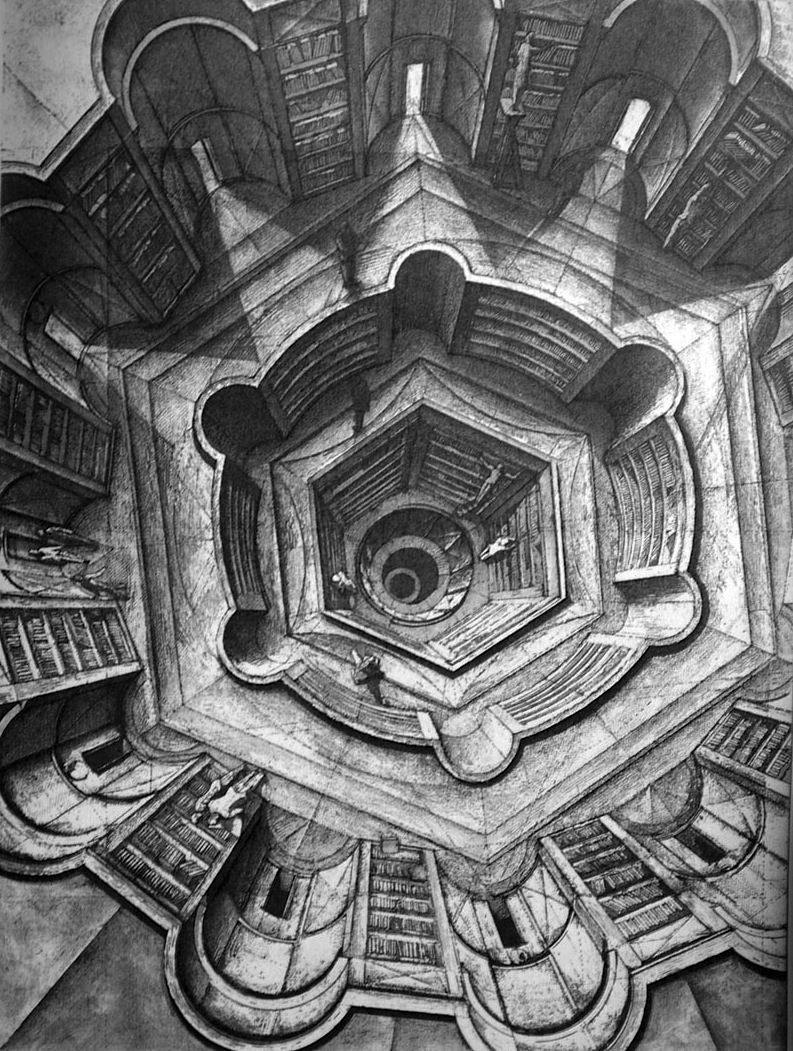
\includegraphics[width=.9\textwidth]{babel.jpg}
    \end{figure}
  \end{columns}

\end{frame}

% ----------------------------------------------------------------------------

\begin{frame}{Normalidad y discrepancia}

  \begin{itemize}
    \item Definimos la \emph{discrepancia} de una sucesión como
    \[
      \discrepancy{N}((x_n)_{n \geq 0})
      = \sup_{\gamma \in (0,1]} \left\vert
        \frac{\# \lbrace 0 \leq n < N \;\vert\; \lbrace x_n \rbrace < \gamma \rbrace}
        {N} - \gamma
      \right\vert.
    \]
    \item Un número $\alpha$ es normal en base $b$ si
    \[ \discrepancy{N}(\lbrace \alpha b^n \rbrace_{n\geq0})
    \xrightarrow{N \to \infty} 0. \]
    \item La discrepancia cuantifica con qué velocidad un número converge a
    la normalidad.
  \end{itemize}

\end{frame}

% ----------------------------------------------------------------------------

\begin{frame}{Construyendo números normales}
  \begin{itemize}
    \item M. Levin definió un número normal basado en el triángulo de Pascal
    con una discrepancia de
    \[ \Ord \left(\frac{\log^2(N)}{N}\right), \]
    la mínima conocida por el momento.
    \pause
    \item V. Becher y O. Carton generalizaron el resultado concatenando
    secuencias perfectas anidadas.
    \begin{itemize}
      \item Sea $\alpha \in [0, 1)$ tal que su escritura en base $b$ es ${,}w_0 w_1 w_2 \dots$, \\ con cada $w_k$ una secuencia $(2^k,2^k)$-perfecta anidada.
      \item $\alpha$ es normal en base $b$,
      y su discrepancia es del mismo orden que la del número de Levin.
    \end{itemize}
    \pause
    \item En esta tesis generalizamos este resultado a la concatenación
    de secuencias maravillosas anidadas.
  \end{itemize}
\end{frame}

% ----------------------------------------------------------------------------

\begin{frame}{Nuestra construcción}
  \begin{itemize}
    \item Sea $\alpha \in [0, 1)$ tal que su escritura en base $b$ es
    \[ {,}w_0w_1w_2\dots \]
    con cada $w_k$ una secuencia $(q^k, \varphi(q^k))$-maravillosa anidada,  \\ siendo:
    \begin{itemize}
      \item $q \geq 2$ un entero,
      \item $\varphi: \nats \to \nats$ una función creciente.
    \end{itemize}
    \item Si $\varphi(\log(N)) = \ord(N)$, $\alpha$ es normal en base $b$ con
      \[ \discrepancy{N}(\lbrace \alpha b^n \rbrace)_{n\geq0}
      = \Ord\left( \frac{\varphi(\log(N))\log(N)}{N} \right). \]
    \item $\varphi$ representa la relación entre los parámetros $n$ y $m$.
      \begin{itemize}
        \item Si es lineal, la discrepancia es $\Ord \left(\log^2(N)/N\right)$.
        \item Si es cuadrática, la discrepancia es $\Ord \left(\log^3(N)/N\right)$.
        \item En general, si $\varphi = \Ord(N^c)$, la discrepancia es $\Ord \left(\log^{c+1}(N)/N\right)$.
      \end{itemize}
  \end{itemize}
\end{frame}

% ============================================================================

\end{document}
